\documentclass{article}


% preambulo:
% ! Tex root = mecat-motor-main

\usepackage[utf8]{inputenc}
% caracteres utf8 (tildes, enie) sin tener que usar comandos



\usepackage[T1]{fontenc}

\usepackage[spanish, es-tabla, es-nodecimaldot]{babel} 
% texto automatico en espaniol
% "tabla" en vez de "cuadro"
% no reemplaza puntos decimales por comas

%% NO AGREGAR PAQUETES ANTES DE ESTO, ES IMPORTANTE QUE BABEL ESTE PRIMERO

%%%%%%%%%%%%%%%%%%%%%%%%%%%%%%%%%
%% PAQUETES EXTRA %%%%%%%%%%%%%%%
%%%%%%%%%%%%%%%%%%%%%%%%%%%%%%%%%

\usepackage{hyperref}					% Hyperlinks on pdf (must be called before Geometry)

\usepackage[a4paper, total={6in, 9in}, footskip=25px]{geometry} 

\usepackage{sansmathfonts}				% Sans Serif equations

\renewcommand*\familydefault{\sfdefault} 	% Sans Serif as default font



\usepackage{subfiles}
\usepackage{xr} % permite referencias a labels de archivos externos con \externaldocument{filename.tex}

\usepackage{amsmath} % PAQUETES DE MATEMATICA
\usepackage{amsfonts}
\usepackage{amssymb}


\usepackage{booktabs} % tablas lindas

\usepackage{units} % permite usar nicefrac
\usepackage{siunitx}
\usepackage{graphicx} % importar imagenes
\usepackage{float} % posicion H para floats
\usepackage[colorinlistoftodos]{todonotes}


\setlength{\parindent}{10pt}			%cuanta sangria al principio de un parrafo
\usepackage{indentfirst}				%pone sangria al primer parrafo de una seccion


% Header style
\usepackage{fancyhdr}
\setlength{\headheight}{15.2pt}
\pagestyle{fancy}
\lhead{31.99 Mecatr\'onica Aplicada}
\chead{TP Motor}
\rhead{Roc\'io Parra}
\cfoot{\thepage}


%\usepackage{dblfnote}
%\DFNalwaysdouble 


\hypersetup{
	colorlinks=true,
	linkcolor=blue,
	filecolor=magenta,      
	urlcolor=blue,
	citecolor=blue,    
}

%Para los graficos con multiples imagenes en el mismo float
\usepackage{caption}
\usepackage{subcaption}

\usepackage{wrapfig} % figuras wrappeadas por texto
\usepackage{verbatim} % comment and verbatim environments

\usepackage{listings}
\usepackage{xcolor}

\definecolor{codegreen}{rgb}{0,0.6,0}
\definecolor{codegray}{rgb}{0.5,0.5,0.5}
\definecolor{codepurple}{rgb}{0.58,0,0.82}
\definecolor{backcolour}{rgb}{0.95,0.95,0.92}


\lstdefinestyle{mystyle}{
	backgroundcolor=\color{white},   
	commentstyle=\color{codegreen},
	keywordstyle=\color{magenta},
	numberstyle=\tiny\color{codegray},
	stringstyle=\color{codepurple},
	basicstyle=\ttfamily\footnotesize,
	breakatwhitespace=false,         
	breaklines=true,                 
	captionpos=b,                    
	keepspaces=true,                 
	numbers=left,                    
	numbersep=5pt,                  
	showspaces=false,                
	showstringspaces=false,
	showtabs=false,                  
	tabsize=2
}

\lstset{style=mystyle}

 



\begin{document}

%\newgeometry{total={6in, 8in}, footskip=50px} % margenes default para la caratula
% caratula:
% !Tex root = mecat-motor-main

\begin{titlepage}
\newcommand{\HRule}{\rule{\linewidth}{0.5mm}}
\center
\mbox{\textsc{\LARGE \bfseries {Instituto Tecnol\'ogico de Buenos Aires}}}\\[1.5cm]
\textsc{\Large 31.99 Mecatr\'onica Aplicada}\\[0.5cm]


\HRule \\[0.6cm]
{ \Huge \bfseries Trabajo Pr\'actico:  

 Control discreto de un motor DC
%
%Realimentados\vspace{0.2cm} 
 }\\[0.4cm] % Title of your document
\HRule \\[1.5cm]

\vfill
{\large

%\emph{Grupo 2}\\
%\vspace{3px}

\begin{tabular}{lr} 	
\textsc{Parra}, Roc\'io  & 57669 \\
\end{tabular}

\vspace{50px}

\emph{Profesores}\\
\vspace{3px}
\textsc{Perfumo}, Lucas Alberto\\ 
\textsc{Fortunatti}, Nelson Ariel\\
\vspace{100px}

\begin{tabular}{ll}

Presentado: & 15/11/2020\\


\end{tabular}

}

\vfill

\end{titlepage}

%\newgeometry{a4paper, total={7in, 9.25in}, footskip=25px}
%\newpage

\section{Modelado del motor}

Para modelar la planta constituida por el motor, se analiz\'o su respuesta a un escal\'on de referencia, desde el reposo hasta la velocidad nominal de 290rpm. La medici\'on se puede observar en la \autoref{fig:lazoabierto}.

\begin{figure}[ht]
	\centering
	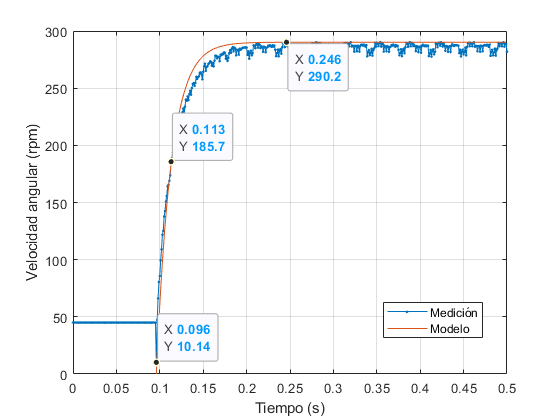
\includegraphics[scale=0.75]{imgs/lazoabierto.png}
	\caption{Respuesta al escal\'on a lazo abierto}
	\label{fig:lazoabierto}
\end{figure}

La respuesta obtenida es aproximadamente consistente con la de un sistema de primer orden (una exponencial creciente), como se muesta en la curva roja. Bajo esta suposici\'on, obtener el modelo del motor es equivalente a obtener las constantes $K$ y $\tau$ tales que
\begin{equation}
	P(s) = \frac{K}{s\cdot\tau+1},
\end{equation} 
donde $P(s)$ es la respuesta en frecuencia en tiempo continuo del motor (la planta que se est\'a estudiando).

Esta planta recibe como entrada una tensi\'on en V, y se obtiene como salida una velocidad en rpm.

La respuesta a un escal\'on entre 0V y 12V, es decir la se\~nal medida, debe bajo este modelo corresponder a la siguiente f\'ormula:
\begin{equation}
	y(t) = K\cdot 12\si\volt \cdot (1 - e^{ -\nicefrac{(t-t_0)}{\tau}}),
\end{equation}
donde $t_0$ es el instante en el cual se aplica el escal\'on de entrada, y se obtiene por simple inspecci\'on del gr\'afico.

Para obtener $K$, basta despejarla del valor final de la salida:
\[
	\lim_{t\to\infty}y(t) = K\cdot 12\si\volt \simeq 290.2\,\text{rpm}
\]
\begin{equation}
	\Rightarrow K = \frac{290.2\,\text{rpm}}{12\si\volt} 
	\simeq  3.55\,\nicefrac{\text{rpm}}{\si\volt}
\end{equation}

Para obtener $\tau$, usamos la propiedad de sistemas de primer orden: $y(\tau) = (y_{final}-y_0)\cdot(1-e^{-1})$ y buscamos el $t$ cuyo $y(t)$ sea lo m\'as cercano posible a este valor. Se obtiene as\'i:
\begin{equation}
	\tau = 0.017\si\second
\end{equation}

Con estas dos constantes se obtiene la curva roja que se observa en la \autoref{fig:lazoabierto}, y se considera que el modelo es suficientemente cercano al comportamiento medido para proceder con el dise\~no del controlador.



\section{Control PID}

Se propone cerrar el lazo de control utilizando un controlador PID. Se busca satisfacer las siguientes condiciones:
\begin{equation}
	\begin{cases}
		M_P &< 10 \% \\
		t_s &< 1.5\si\second
	\end{cases}
\end{equation}

Un controlador PID gen\'erico es de forma:
\begin{equation}
	C(s) = k_p + k_d\cdot s + \nicefrac{k_i}{s}
\end{equation}

Como el sistema a lazo abierto responde en aproximadamente 150ms (es decir, mucho m\'as r\'apido de lo que se pide), no parece necesario introducir la complejidad agregada por la parte derivativa del controlador. Adem\'as, se observa en la \autoref{fig:lazoabierto} que hay un ruido considerable en las mediciones, que se ver\'ia amplificado por la derivaci\'on. Por lo tanto, se define $k_d = 0$.

Para elegir el valor de las otras constantes, se calcula la transferencia a lazo cerrado del sistema:
\begin{equation}
	T(s) = \frac{P(s)\cdot C(s)}{1+P(s)\cdot C(s)}
	= 
	\frac{
		K \cdot k_p /\tau \cdot \left(s+\nicefrac{k_i}{k_p}\right)
	}{
		s^2 + (1+K\cdot k_p)/\tau \cdot s + K\cdot k_i/ \tau 
	}
\end{equation}

Este sistema tiene un cero en el semiplano izquierdo, en frecuencia $k_i/k_p$, y dos polos con par\'ametros:
\begin{equation}
	\begin{cases}
		\omega_0^2 &= \frac{K\cdot k_i}{\tau} \\
		2\xi\omega_0 &= \frac{1+K\cdot k_p}{\tau}  
	\end{cases}
\end{equation}

Para seleccionar $k_i$ y $k_p$, se asumir\'a inicialmente que la respuesta est\'a \'unicamente determinada por los polos, y luego se ajustar\'a $k_p$ heur\'isticamente para cumplir los requerimientos establecidos. Esto permite reducir el sobrepico, pero tambi\'en hace que el sistema responda m\'as lento, con lo cual se partir\'a de $t_s=1\si\second$ y $m_p=0.01$ para contar con un margen de error.

A partir de estas condiciones se pueden obtener los $\xi$ y $\omega_0$ deseados:
\begin{equation}
	\begin{cases}
		\xi = \frac{-\ln(m_p)}{\sqrt{\pi^2 + 
		\ln^2{(m_p)}}} &\simeq 0.8261 \\
		\omega_0 = \frac{4}{\xi\cdot t_s} &\simeq 4.8421\nicefrac{rad}{s} 
	\end{cases}
\end{equation}

A partir de estos valores, se pueden despejar $k_i$ y $k_p$. Se ajust\'o $k_p$ con un factor de 1.5 para complir la especificaci\'on. Se obtiene entonces:
\begin{equation}
	\begin{cases}
		k_i = \frac{\omega_0^2\cdot\tau}{K} &\simeq 387.9655\\
		k_p = 1.5\cdot \frac{2\xi\omega_0\cdot\tau-1}{K} &\simeq 198.1436  
	\end{cases}
\end{equation}

Queda as\'i completamente definido el controlador PID en tiempo continuo. Para implementar su versi\'on discreta, se utiliz\'o la aproximaci\'on de Tustin. El resultado se observa en la \autoref{fig:lazocerrado}

\begin{figure}[ht]
	\centering
	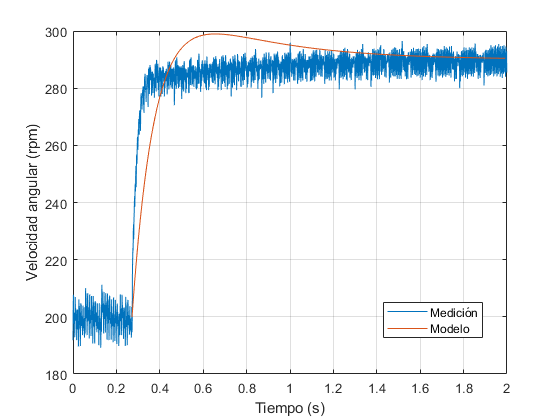
\includegraphics[scale=0.75]{imgs/lazocerrado.png}
	\caption{Respuesta al escal\'on a lazo cerrado}
	\label{fig:lazocerrado}
\end{figure}

Las mediciones indican que el sistema funciona en r\'egimen sobreamortiguado, con lo cual el requerimiento de m\'aximo overshoot es ampliamente satisfecho. En general, la desventaja de esta caracter\'istica es un tiempo de establecimiento mayor, pero tambi\'en este par\'ametro es adecuado de acuerdo a la especificaci\'on.

Esto se debe en gran parte a que el sistema funcionaba pr\'acticamente dentro de especificaci\'on por s\'i mismo: su tiempo de respuesta era 10 veces menor al requerido, y no presentaba sobrepico. Sin embargo, el control integral permite eliminar el error permanente, lo cual no pod\'ia garantizarse a lazo abierto.

\end{document}
